% Design: publish and attach as operations on mappings. On the left, what a
% publisher hands over: a state file with the tokens and the cells of the
% prefix (16 bytes per token) and without its rows. On the right, the rows,
% which stay in place: the publisher changes the protection of its entries
% (after the device has completed its writes), and an agent maps the same
% pages read-only and reads them from the CPU, which sets the accessed flags.
% What a process writes afterwards lies in pages of its own.
\documentclass[border=2pt]{standalone}
% Shared TikZ style of the STATOR design figures. Teal marks shared,
% immutable state; amber marks what one process writes; violet marks a
% second level of sharing; text is regular weight except the panel titles.
\usepackage{newtxtext}
\usepackage{tikz}
\usetikzlibrary{arrows.meta, positioning, fit, calc, patterns, shapes.geometric, decorations.pathreplacing}

\definecolor{panel}{HTML}{F3F4F6}   % a group of components
\definecolor{gpuc}{HTML}{E4E0F6}    % the GPU
\definecolor{ptc}{HTML}{FAF0DC}     % page tables and the SMMU
\definecolor{modelc}{HTML}{CDEBE6}  % the weights
\definecolor{sharedc}{HTML}{7FCBC1} % shared rows, read-only
\definecolor{tailc}{HTML}{F7B955}   % rows of one process, in use
\definecolor{aheadc}{HTML}{FCE6C2}  % populated ahead, or write-protected
\definecolor{copyc}{HTML}{F4BFCB}   % a copied page
\definecolor{segc}{HTML}{B7A9E8}    % the segment of a second ancestor
\definecolor{faultc}{HTML}{E8736A}  % a private copy made by a fault
\definecolor{actc}{HTML}{FDE9C9}    % an operation of the design
\definecolor{roline}{HTML}{14786F}  % read-only mappings
\definecolor{rwline}{HTML}{C5432F}  % writable mappings and faults

\tikzset{
  layer/.style={draw=black!60, fill=panel, line width=0.5pt},
  sub/.style={draw=black!55, line width=0.4pt},
  comp/.style={draw=black!85, fill=white, line width=0.4pt, align=center,
               font=\scriptsize, inner xsep=3pt, inner ysep=1.5pt, minimum height=0.5cm},
  seg/.style={draw=black!65, line width=0.35pt, inner sep=0pt, align=center,
              font=\scriptsize, minimum height=0.4cm},
  free/.style={seg, pattern=north east lines, pattern color=black!40},
  blk/.style={draw=black!65, line width=0.35pt, minimum width=0.42cm, minimum height=0.36cm,
              inner xsep=2pt, inner ysep=0pt, font=\scriptsize},
  hole/.style={blk, pattern=north east lines, pattern color=black!45},
  tag/.style={font=\scriptsize, inner sep=1pt},
  ttl/.style={font=\bfseries\small},
  lbl/.style={font=\scriptsize},
  note/.style={font=\itshape\scriptsize, inner sep=1pt},
  arr/.style={-{Latex[length=1.6mm]}, line width=0.8pt},
  thin/.style={-{Latex[length=1.3mm]}, line width=0.5pt},
  fat/.style={-{Triangle[length=2.2mm,width=3.4mm]}, line width=2.4pt},
  num/.style={circle, fill=black, text=white, font=\bfseries\scriptsize,
              inner sep=0.6pt, minimum size=0.33cm},
}
% A legend entry: a filled square and its name, at (x,y).
\newcommand{\legendfill}[4]{%
  \draw[black!65, line width=0.35pt, fill=#3] (#1,#2) rectangle ++(0.22,0.2);
  \node[tag, anchor=west] at (#1+0.27,#2+0.1) {#4};}
\newcommand{\legendhatch}[3]{%
  \draw[black!65, line width=0.35pt, pattern=north east lines, pattern color=black!45] (#1,#2) rectangle ++(0.22,0.2);
  \node[tag, anchor=west] at (#1+0.27,#2+0.1) {#3};}
% Legend marks for a legend that is one centred line of text:
%   \node[tag] at (x,y) {\lgdfill{sharedc}\,Shared \quad \lgdhatch\,Unbacked};
\newcommand{\lgdfill}[1]{\tikz[baseline=-0.55ex]{\draw[black!65, line width=0.35pt, fill=#1] (0,-0.1) rectangle (0.22,0.1);}}
\newcommand{\lgdhatch}{\tikz[baseline=-0.55ex]{\draw[black!65, line width=0.35pt, pattern=north east lines, pattern color=black!45] (0,-0.1) rectangle (0.22,0.1);}}

\begin{document}
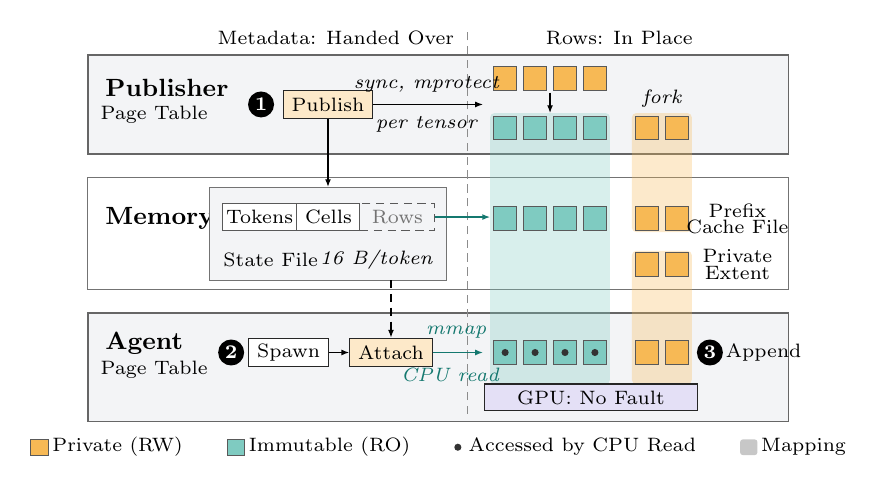
\begin{tikzpicture}[x=1cm, y=1cm,
  tiny/.style={-{Latex[length=1.0mm]}, line width=0.5pt},
  pte/.style={blk, minimum width=0.3cm, minimum height=0.3cm},
  field/.style={seg, minimum height=0.34cm, font=\scriptsize},
  flag/.style={circle, fill=black!80, inner sep=0pt, minimum size=0.09cm}]

% lanes
\draw[layer] (0,4.02) rectangle (8.9,5.28);
\draw[sub, fill=white] (0,2.3) rectangle (8.9,3.72);
\draw[layer] (0,0.62) rectangle (8.9,2.0);
\node[ttl, anchor=west] at (0.1,4.86) {Publisher};
\node[tag, anchor=west] at (0.12,4.52) {Page Table};
\node[ttl, anchor=west] at (0.1,3.2) {Memory};
\node[ttl, anchor=west] at (0.1,1.62) {Agent};
\node[tag, anchor=west] at (0.12,1.28) {Page Table};

% what is handed over, and what stays in place
\draw[black!45, line width=0.3pt, densely dashed] (4.82,0.72) -- (4.82,5.62);
\node[tag] at (3.15,5.5) {Metadata: Handed Over};
\node[tag] at (6.75,5.5) {Rows: In Place};

% a band joins the entries of a page table with the pages they refer to
\newcommand{\band}[5]{\fill[#1, opacity=0.3, rounded corners=1.5pt] (#2,#3) rectangle (#4,#5);}
\band{sharedc}{5.11}{1.1}{6.63}{4.54}
\band{tailc}{6.91}{3.03}{7.67}{4.54}
\band{tailc}{6.91}{1.1}{7.67}{2.79}

% ---------------- the rows ----------------
% the entries of the publisher: writable while it computes, read-only after
\foreach \k in {0,...,3} {
  \node[pte, fill=tailc] at (5.3+\k*0.38,4.98) {};
  \node[pte, fill=sharedc] at (5.3+\k*0.38,4.35) {};
  \node[pte, fill=sharedc] at (5.3+\k*0.38,3.2) {};
  \node[pte, fill=sharedc] (d\k) at (5.3+\k*0.38,1.5) {};
  \node[flag] at (d\k) {};
}
\draw[tiny] (5.87,4.8) -- (5.87,4.54);
\foreach \k in {0,1} {
  % the rows that the publisher writes after the fork, and their pages
  \node[pte, fill=tailc] at (7.1+\k*0.38,4.35) {};
  \node[pte, fill=tailc] at (7.1+\k*0.38,3.2) {};
  % the private extent of the agent
  \node[pte, fill=tailc] at (7.1+\k*0.38,2.62) {};
  \node[pte, fill=tailc] at (7.1+\k*0.38,1.5) {};
}
\node[note] at (7.29,4.72) {fork};
\node[tag, align=center] at (8.25,3.2) {Prefix\\[-2pt]Cache File};
\node[tag, align=center] at (8.25,2.62) {Private\\[-2pt]Extent};

% ---------------- the metadata ----------------
\node[num] at (2.2,4.65) {1};
\node[comp, fill=actc, minimum width=1.1cm, minimum height=0.36cm, inner ysep=0pt] (publish) at (3.05,4.65) {Publish};
\draw[tiny] (publish.east) -- (5.02,4.65);
\node[note] at (4.3,4.9) {sync, mprotect};
\node[note] at (4.3,4.4) {per tensor};

% the state file: the tokens and the cells of the prefix, and no rows
\draw[sub, fill=panel] (1.55,2.42) rectangle (4.55,3.6);
\node[field, minimum width=0.95cm, fill=white, anchor=west] at (1.7,3.22) {Tokens};
\node[field, minimum width=0.8cm, fill=white, anchor=west] at (2.65,3.22) {Cells};
\node[field, minimum width=0.95cm, densely dashed, anchor=west, text=black!55] (rows) at (3.45,3.22) {Rows};
\node[tag, anchor=west] at (1.68,2.68) {State File};
\node[note, anchor=east] at (4.42,2.68) {16 B/token};
\draw[tiny] (publish.south) -- (3.05,3.6);
\draw[tiny, roline] (rows.east) -- (5.11,3.22);

\node[num] at (1.82,1.5) {2};
\node[comp, minimum width=0.95cm, minimum height=0.36cm, inner ysep=0pt] (spawn) at (2.55,1.5) {Spawn};
\node[comp, fill=actc, minimum width=0.95cm, minimum height=0.36cm, inner ysep=0pt] (attach) at (3.85,1.5) {Attach};
\draw[tiny] (spawn) -- (attach);
\draw[tiny, densely dashed] (3.85,2.42) -- (attach.north);
\draw[tiny, roline] (attach.east) -- (5.02,1.5);
\node[note, text=roline] at (4.68,1.76) {mmap};
\node[note, text=roline] at (4.6,1.22) {CPU read};

% the agent appends in pages of its own; the GPU takes no fault on either kind
\node[num] at (7.9,1.5) {3};
\node[tag, anchor=west] at (8.06,1.5) {Append};
\node[comp, fill=gpuc, minimum width=2.7cm, minimum height=0.34cm, inner ysep=0pt] at (6.39,0.93) {GPU: No Fault};

% legend
\node[tag] at (4.45,0.3) {\lgdfill{tailc}\,Private (RW)\qquad\lgdfill{sharedc}\,Immutable (RO)\qquad\tikz[baseline=-0.55ex]{\node[circle, fill=black!80, inner sep=0pt, minimum size=0.09cm] {};}\,\,Accessed by CPU Read\qquad\tikz[baseline=-0.55ex]{\fill[black!22, rounded corners=1pt] (0,-0.1) rectangle (0.22,0.1);}\,Mapping};
\end{tikzpicture}
\end{document}
